\chapter{Sintassi}

\section{Prologo}

La sintassi è il fenomeno che permette di percepire come corrette certe frasi e come scorrette altre. I linguisti separano la sintassi in:
\begin{itemize}
  \item Competence. 
  \item Performance.
\end{itemize}

\dfn{Competence}{
  La competence rappresenta la grammatica formale. Una conoscenza pura linguistica.
}

\nt{La linguistica dovrebbe occuparsi della competence.}

\dfn{Performance}{
La performance rappresenta un algoritmo di parsing. Come si utilizza la conoscenza pura.
}

\nt{È importante conoscere la grammatica formale per poterla utilizzare con un algoritmo.}

\subsection{Grammatiche Generative}

\dfn{Sistemi di Riscrittura}{
  Sistema formale della tradizione matematica utilizzato come base da Chomsky.
}

\begin{figure}[h]
    \centering
    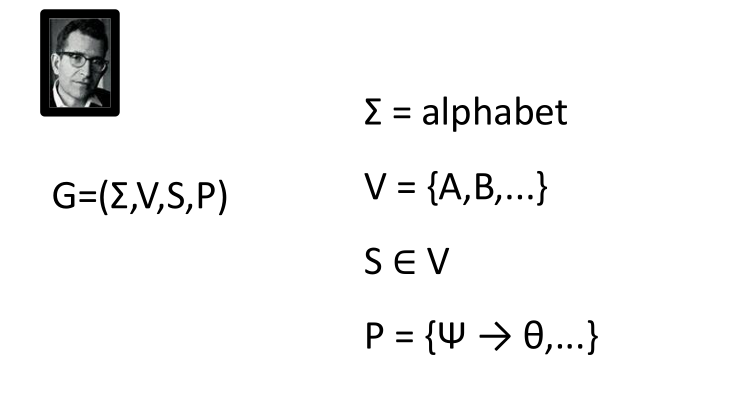
\includegraphics[scale=0.4]{03/gen.png}
    \caption{Grammatiche Generative.}
\end{figure}

\begin{itemize}
  \item Le grammatiche generative modellano il linguaggio naturale come un linguaggio formale. 
  \item L'albero di derivazione può modellare la struttura sintattica della frase. 
\end{itemize}

\paragraph{Le grammatiche context free:}

\begin{itemize}
  \item Costituenza: i costituenti rappresentano i simboli non terminali V. 
  \item Relazione grammaticale. 
  \item Sottocategorigazioni.
\end{itemize}

\nt{Chomsky dimostrò che le lingue naturali sono \fancyglitter{almeno} context free.}

\begin{figure}[h]
    \centering
    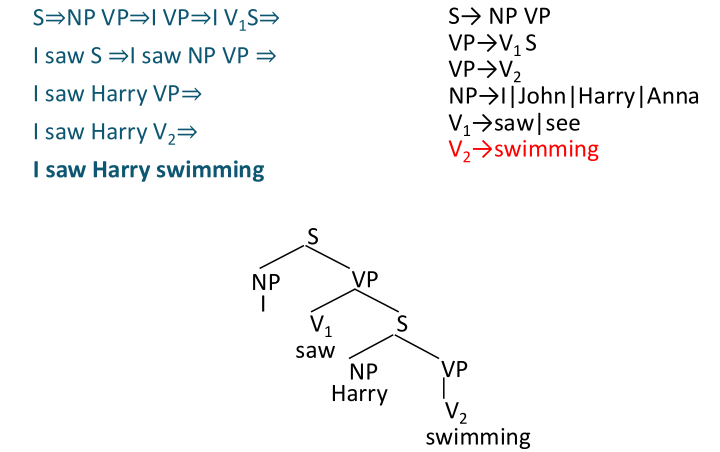
\includegraphics[scale=0.4]{03/esempio.png}
    \caption{Esempio con grammatica giocattolo.}
\end{figure}

\begin{figure}[h]
    \centering
    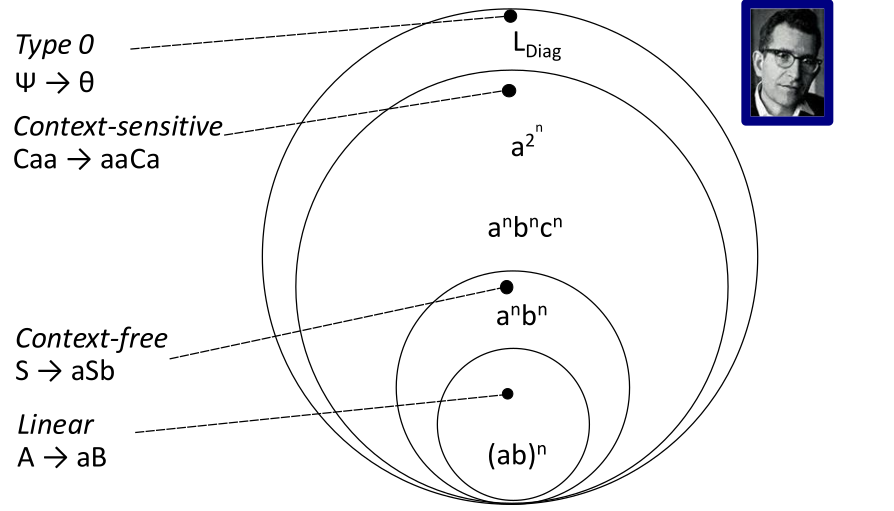
\includegraphics[scale=0.4]{03/chomsky.png}
    \caption{Gerarchia di Chomsky.}
\end{figure}

\nt{Questa gerarchia mette in "ordine" le complessità di vari tipi di linguaggi.
  Le lingue naturali si trovano nel \fancyglitter{context-sensitive}, o meglio, nelle \fancyglitter{mildly-context-sensitive} ($a^n*b^n*c^n$). 
}

\subsection{Mildly-context-sensitive}

\paragraph{Le grammatiche mildly-context-sensitive possiedono quattro proprietà:}

\begin{itemize}
  \item Includono le grammatiche Context-free. 
  \item Hanno dipendenze annidate e incrociate. 
  \item Sono parsificabili polinomialmente. 
  \item Hanno la proprietà di crescita costante.
\end{itemize}

\dfn{Proprietà di Crescita Costante}{
  Un languaggio $L$ cresce costantemente se c'è una costante $c_0$ e un insieme finito di costanti $C$ tale che per ogni $w \epsilon L$ dove $|w| > c_0$ tale che $|w| = |w'| + c$ per qualche $c \epsilon C$. 
}

\nt{Questa proprietà è la versione formale dell'intuizione linguistica che una frase appartenente a un linguaggio naturale può essere costruita da un insieme finito di strutture usando la stessa operazione lineare.}

\begin{figure}[h]
    \centering
    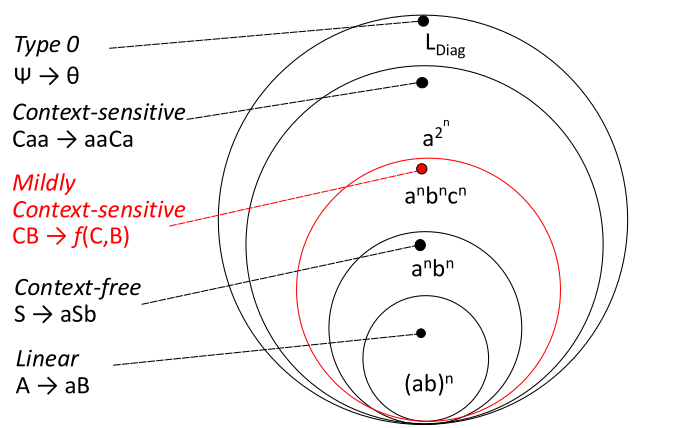
\includegraphics[scale=0.5]{03/mildly.png}
    \caption{Gerarchia di Chomsky con mildly-context-sensitive.}
\end{figure}
\pagebreak
\section{La Performance e i costituenti}

\begin{figure}[!h]
    \centering
    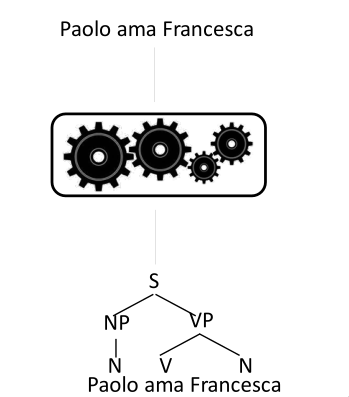
\includegraphics[scale=0.5]{03/parser.png}
    \caption{Un parser trasforma la frase in un albero.}
\end{figure}

\subsection{Approcci al Parsing}

\paragraph{Parser anatomy (Steedman):}

\begin{itemize}
  \item Competence: Context-free, TAG, CCG, Dipendenza, etc.
  \item Algoritmo: 
    \begin{itemize}
      \item Strategia di ricerca: top-down, bottom-up, left-to-right, etc. 
      \item Organizzazione della memoria: back-tracking (approccio in profondità, PROLOG), programmazione dinamica (approccio in ampiezza).
    \end{itemize}
  \item Oracolo: probabilistico, a regole, etc.
\end{itemize}

\nt{L'oracolo serve per via dell'ambiguità delle lingue naturali. Decide quale regola applicare prima secondo suoi criteri.}

\paragraph{Fonti di informazioni:}

\begin{itemize}
  \item Grammatica $\rightarrow$ parsing diretto dai goal $\rightarrow$ top-down. 
    \begin{itemize}
      \item Solo ricerche che possono portare a risposte corrette, cioè con
radice S. 
      \item Comporta la creazione di alberi non compatibili con le parole. 
      \item Razionalisti.
    \end{itemize}
  \item Frase $\rightarrow$ parsing diretto dai dati $\rightarrow$ bottom-up. 
    \begin{itemize}
      \item Solo ricerche compatibili con le parole. 
      \item Comporta la creazione di alberi non corretti. 
      \item Empiristi.
    \end{itemize}
\end{itemize}

\paragraph{Parser A:}

\begin{itemize}
  \item Context-free. 
  \item Top-down, left-to-right, back-tracking. 
  \item Rule-based.
\end{itemize}

\paragraph{Problemi del parser A:}

\begin{itemize}
  \item È lento: prova tutte le combinazioni e fa back-tracking. 
  \item Va in loop: a causa della ricorsione se sono presenti regole che vanno in sé stesse.
\end{itemize}

\qs{}{Come ri gestisce l'esplosione combinatoria dei sottoalberi?}

\paragraph{Con la programmazione dinamica (Richard Bellman):}

\begin{itemize}
  \item Sottostrutture ottimali. 
  \item Sottoproblemi sovrapponibili. 
  \item Memoizzazione.
\end{itemize}

\dfn{CKY}{
  Calcola tutti i possibili parse in tempo $O(n^3)$. Il difetto maggiore è che il
caso peggiore e il caso medio coincidono (ma anche esige una forma normale per la
grammatica).
}

\nt{Questo algoritmo fu scoperto da tre persone nel giro di un anno e mezzo: Cocke, Kasami e Younger.}

\paragraph{Parser B (CKY):}

\begin{itemize}
  \item Context-free. 
  \item Bottom-up, left-to-right, programmazione dinamica. 
  \item Rule-based.
\end{itemize}

\paragraph{Idea del CKY:}

\begin{itemize}
  \item Salva i sottoalberi perché possono essere riutilizzati. 
  \item Si rende in forma normale di Chomsky (solo regole binarie): 
    \begin{itemize}
      \item Si copiano tutte le regole binarie nella nuova grammatica, senza cambiarle. 
      \item Si convertono i terminali in non terminali. 
      \item Si binarizzano tutte le regole e si aggiungono alla nuova grammatica.
    \end{itemize}
\end{itemize}

\paragraph{A $\rightarrow$ BC:}

\begin{enumerate}
  \item Se c'è un A allora c'è un B seguito da un C. 
  \item Se A va da $i$ a $j$, c'è un $k$ tale che $i < k < j$. 
  \item Cioè B va da $i$ a $k$ e C va da $k$ a $j$. 
  \item Usiamo una matrice per mettere B in matrix$[i,k]$, C in matrix$[k,j]$, A in matrix$[i,j]$. 
  \item Loop su $k$. 
  \item Se il parsing ha successo S è in $[0, n]$.
\end{enumerate}

\begin{figure}[!h]
    \centering
    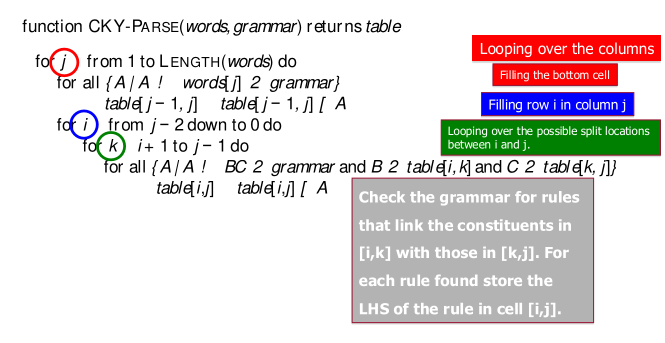
\includegraphics[scale=0.5]{03/CKY.png}
    \caption{Algoritmo del CKY.}
\end{figure}

\paragraph{Complessità:}

\begin{itemize}
  \item $O(n^3)$. 
  \item $O(n^5)$ nella versione probabilistica. 
  \item Troppo lento per il real-time (motori di ricerca). 
\end{itemize}

\subsection{Parsing Probabilistico}

\paragraph{Parser C (CKY probabilistico):}

\begin{itemize}
  \item Probabilistic Context-free. 
  \item Bottom-up, left-to-right, programmazione dinamica. 
  \item Probabilistico.
\end{itemize}

\begin{figure}[!h]
    \centering
    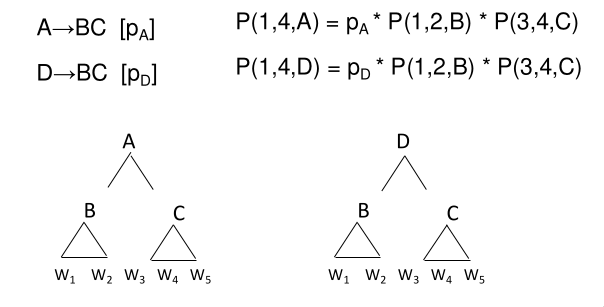
\includegraphics[scale=0.55]{03/prob.png}
    \caption{CKY probabilistico.}
\end{figure}

\nt{Per fare ciò si realizza una distribuzione probabilistica sulle regole della grammatica.}

\qs{}{Da dove si prendono le probabilità?}

\begin{itemize}
  \item Treebanks $\rightarrow$ Banche di alberi:
    \begin{itemize}
      \item Costituenti $\rightarrow$ Penn TB. 
      \item Dipendenze $\rightarrow$ TUT TB $\rightarrow$ Universal Dependency TB.
    \end{itemize}
  \item Si creano con sistemi semiautomatici: 
    \begin{itemize}
      \item Prima con un parser. 
      \item Successivamente si corregge a mano.
    \end{itemize}
  \item Guidelines di annotazione. 
  \item Corpus Linguistics.
\end{itemize}

\nt{I Treebanks sono più costosi del PoS.}

\paragraph{Training del modello probabilistico:}

\begin{itemize}
  \item Serve $P(\alpha \rightarrow \beta | \alpha)$. 
  \item Quindi per ogni albero nel TB si calcola: 
    $$P(\alpha \rightarrow \beta | \alpha) = \frac{\text{Count}(\alpha \rightarrow \beta)}{\sum_\gamma \text{Count}(\alpha \rightarrow \gamma)} = \frac{\text{Count}(\alpha \rightarrow \beta)}{\text{Count}(\alpha)}$$
\end{itemize}

\begin{figure}[!h]
    \centering
    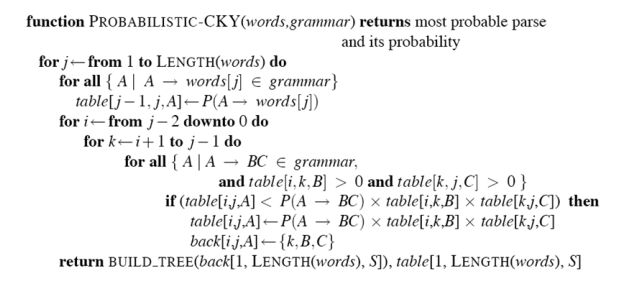
\includegraphics[scale=0.5]{03/PCKY.png}
    \caption{Algoritmo del CKY probabilistico.}
\end{figure}

\nt{Attualmente si usano anche oracoli neurali dando vita a CKY neurali.}

\subsection{Valutazione}

\begin{itemize}
  \item Precision: 
    \begin{itemize}
      \item Quale percentuale di subtree del system tree sono anche nel gold tree?
      \item Quanto di quello prodotto è giusto?
    \end{itemize}
  \item Recall:
    \begin{itemize}
      \item Quale percentuale di subtree del golden tree sono anche nel system tree?
      \item Quanto di quello che avremmo dovuto produrre abbiamo realmente prodotto?
    \end{itemize}
\end{itemize}

\begin{figure}[!h]
    \centering
    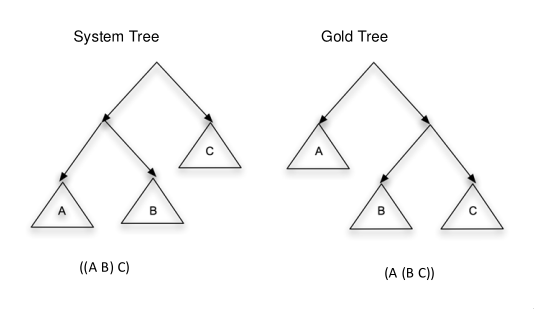
\includegraphics[scale=0.45]{03/stgt.png}
    \caption{System tree e Gold tree.}
\end{figure}

\paragraph{Problema con i parser probabilistici:}

\begin{itemize}
  \item Non ci sono preferenze lessicali.
\end{itemize}

\nt{Per questo motivo si utilizzano dei parser probabilistici \fancyglitter{lexicalized} in cui si tiene anche conto dell'informazione lessicale. Purtroppo facendo così aumentano il numero di regole.}

\subsection{Parsing Parziale}

\paragraph{Parser E (Chunk parsing a regole):}

\begin{itemize}
  \item Regular-Grammars (cascade). 
  \item Bottom-up, programmazione dinamica. 
  \item Rule-based.
\end{itemize}

\nt{Si rimuove la ricorsione. I sintagmi possono essere ricorsivi, i chunk (unità sintattiche di base) no.}

\section{Parsing a Dipendenze}

\begin{figure}[!h]
    \centering
    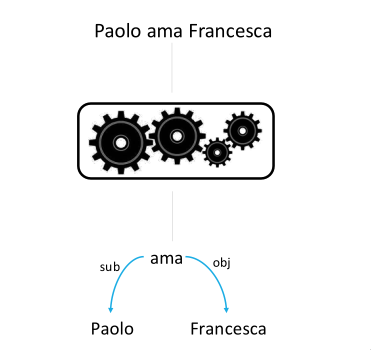
\includegraphics[scale=0.45]{03/parser a dipendenze.png}
    \caption{Un parser a dipendenze.}
\end{figure}

\subsection{Sintassi a Dipendenze}

\dfn{Sintassi a Dipendenze}{
  La sintassi a dipendenze postula che la struttura
sintattica consiste di elementi lessicali connessi da
relazioni binarie asimettiche (graficamente frecce)
chiamate \newfancyglitter{dipendenze}.
}

\nt{Non ci sono relazioni alla pari, c'è sempre un soggetto passivo e uno attivo.}

\begin{figure}[!h]
    \centering
    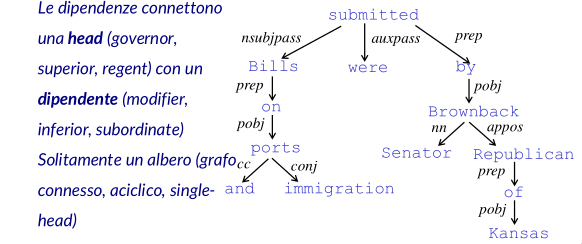
\includegraphics[scale=0.45]{03/dip.png}
    \caption{Esempio di sintassi a dipendenza.}
\end{figure}

\qs{}{Cosa è una testa (head)?}

\begin{itemize}
  \item H determina la categoria sintattica di C; H puo sostituire C. 
  \item H è obbligatoria; D può essere opzionale. 
  \item H seleziona D e determina quando D è obbligatoria. 
  \item La forma di D dipende da H (agreement). 
  \item La posizione nella frase di D è specificabile con
riferimento a H. 
\item H detemina la categoria semantica di C.
\end{itemize}

\clm{}{}{
  \begin{itemize}
    \item H: Head. 
    \item D: Dependent. 
    \item C: Costruzione.
  \end{itemize}
}

\paragraph{Vantaggi delle dipendenze:}

\begin{itemize}
  \item Generalizzazioni tra lingue. 
  \item Predizione psicolinguistica.
  \item Trasparenza e semplicità di rappresentazione.
\end{itemize}

\paragraph{Svantaggi delle dipendenze:}

\begin{itemize}
  \item L'assunzione di relazioni binarie asimmetriche non è sempre corretto (e. g. Cani e gatti).
\end{itemize}

\nt{Le relazioni tra head e dipendenze sono una buona approssimazione della relazione tra predicati e i loro argomenti.}

\subsection{Approcci}

\paragraph{Tecniche per il dependency parsing:}

\begin{itemize}
  \item Programmazione dinamica. 
  \item Algoritmi per i grafi. 
  \item Parsing a costituenza. 
  \item Parsing transition-based. 
  \item Constrain Satisfaction.
\end{itemize}

\dfn{Dynamic Parsing}{
  Utilizza la programmazione dinamica (simile a CKY). L'algoritmo è simile al parsing delle PCFG lessicalizzate (con complessità $O(n^5)$). 
}

\begin{figure}[!h]
    \centering
    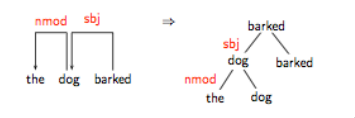
\includegraphics[scale=0.7]{03/dynamic.png}
    \caption{Dynamic Parsing.}
\end{figure}

\clm{}{}{
  \begin{itemize}
    \item Dynamic Programming.
    \item Eisner (1996) ha scoperto un algoritmo migliore che riduce la complessità a $O(n^3)$.
  \end{itemize}
}

\dfn{Graph Algorithms}{
  Si crea un minimum spanning tree per la frase. Le dipendenze vengono valutate usando un ML Classifier.
}

\begin{figure}[!h]
    \centering
    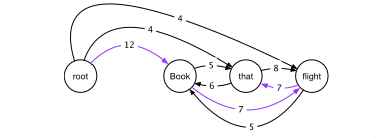
\includegraphics[scale=0.7]{03/graph.png}
    \caption{Graph Algorithm.}
\end{figure}

\nt{Il primo algoritmo del motore di ricerca Google aveva un parsing di questo tipo.}

\dfn{Constituency Parsing}{
  Parsing con una grammatica a costituenti e converto in un formato a
dipendenze attraverso delle “tabelle di percolazioni” (teoria X-bar). Scelte greedy per la creazione di dipendenze tra parole, guidate da
ML classifiers. Vengono eliminate tutte le possibili dipendenze che non soddifano a
certi vincoli.
}

\dfn{Deterministic Parsing}{
  Si fanno scelte greedy per la creazione di dipendenze tra parole, guidate da ML classifiers. Possono essere transition-based.
}

\dfn{Constraint Satisfaction}{
  Vengono eliminate tutte le dipendenze che non soddisfano a certi vincoli.
}

\subsection{Parsing Deterministico a Transizioni}

\paragraph{Parser F (MALT):}

\begin{itemize}
  \item Dependency grammar. 
  \item Bottom-up, depth-first. 
  \item Probabilistico.
\end{itemize}

\begin{figure}[!h]
    \centering
    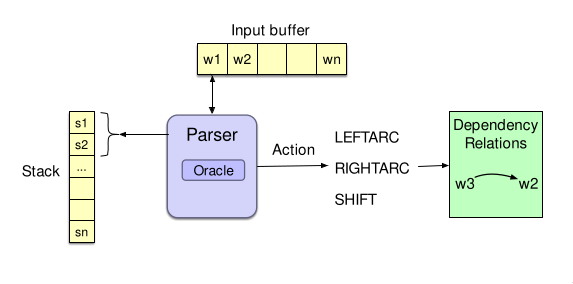
\includegraphics[scale=0.45]{03/parserf.png}
i    \caption{Transition-based parsing.}
\end{figure}

\cor{Proiettività}{
  IF $i \rightarrow j$ THEN $i \rightarrow * k$ for any $k$ such that $i<k<j$ or $j<k<i$.
}

\nt{In parole povere: se non ci sono incroci.}

\begin{figure}[!h]
    \centering
    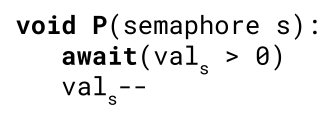
\includegraphics[scale=0.85]{03/P.png}
    \caption{Struttura proiettiva.}
\end{figure}

\begin{figure}[!h]
    \centering
    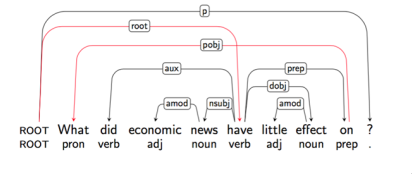
\includegraphics[scale=0.8]{03/NP.png}
    \caption{Struttura non proiettiva.}
\end{figure}


\clm{}{}{
  \begin{itemize}
    \item La maggior parte dei framework non assume la proiettività. 
    \item Le strutture non proiettive sono necessarie per tenere conto delle dipendenze a lunga distanza (e. g. le domande).
  \end{itemize}
}

\paragraph{Uno \fancyglitter{stato} è composto da tre cose:}

\begin{itemize}
  \item Uno stack che contiene le parole parzialmente analizzate. 
  \item Una lista contenente le rimanenti parole da analizzare. 
  \item Un insieme contenente le dipendenze create fino a quel punto nell'analisi.
\end{itemize}

\paragraph{Stato iniziale:}

\begin{itemize}
\item \{$[$root$]$, $[$sentence$]$, ()\}.
\end{itemize}

\paragraph{Stato finale:}

\begin{itemize}
\item \{$[$root$]$, $[$$]$, (R)\}.
\item R è l'insieme delle dipendenze costruite. 
\item $[]$ è la lista vuota poiché tutte le parole sono state analizzate.
\end{itemize}

\clm{Operatori di parsing}{}{
  \begin{itemize}
    \item LeftArc: asserisce una relazione testa-dipendenza tra la parola sulla cima dello stack e la seconda parola nello stack (rimuove la seconda parola dallo stack). 
    \item RightArc: asserisce una relazione testa-dipendenza tra la seconda parola nello stack e la parola sulla cima dello stack (rimuove la cima dallo stack). 
    \item Shift: rimuove la parola dall'inizio dell'input e fa "push" sullo stack.
  \end{itemize}
}

\begin{figure}[!h]
    \centering
    \includegraphics[scale=0.8]{03/DP.png}
    \caption{Algoritmo per fare il parsing delle dipendenze.}
\end{figure}

\nt{Questo algoritmo è greedy: l'oracolo fornisce una singola scelta a ogni step e il parser procede con quella scelta (non c'è back-tracking).}

\paragraph{\fancyglitter{2 Problemi:}}

\begin{enumerate}
  \item Operatori e dipendenze: come tipare?
  \item Quale operatore (L, R, S) si deve utilizzare a ogni passo? Bisogna avere un buon oracolo.
\end{enumerate}

\paragraph{Problema 1:}

\begin{itemize}
  \item $n$ dipendenze $\rightarrow 2^n + 1$ operatori, ossia Left e Right in combinazione con tutte le relazioni + Shift.  
\end{itemize}

\paragraph{Problema 2:}

\begin{itemize}
  \item Oracolo a regole: si sceglie l'operatore da applicare usando un insieme di regole sul valore delle features dello stato corrente. 
  \item Oracolo Probabilistico: si usa un sistema di ML per addestrare un classifier per scegliere l'operatore.
\end{itemize}

\clm{}{}{
Per usare il ML bisogna: 
\begin{itemize}
  \item Trovare le features linguisticamente significative. 
  \item Costruire il training data. 
  \item Implementare un training algorithm.
\end{itemize}
}

\paragraph{Trovare le features:}

\begin{itemize}
  \item A mano. 
  \item In modo automatico utilizzando un classificatore neurale.
\end{itemize}

\paragraph{Training Data:}

\begin{itemize}
  \item TB (Treebank) a dipendenze. 
  \item TB a costituenti e conversione (percolazione).
\end{itemize}

\paragraph{Training Algorithm:}

\begin{itemize}
  \item Dato un albero del TB si devono ricostruire tutte le scelte giuste del parser per costruire quello specifico albero. 
  \item Si usa questo algoritmo: 
    \begin{itemize}
      \item LeftArc: se ottengo la dipendenza che correttamente si trova nell'albero. 
      \item RightArc: se ottengo la dipendenza che correttamente si trova nell'albero e tutte le altre dipendenze associate alla parola figlia si trovano già nell'albero. 
      \item Shift: in tutti gli altri casi.
    \end{itemize}
\end{itemize}

\subsection{Parsing a Regole per Dipendenze a Vincoli}

\paragraph{Parser G (TUP, Turin University Parser):}

\begin{itemize}
  \item Dependency grammar (constrains). 
  \item Bottom-up, depth-first. 
  \item Rule-based.
\end{itemize}

\paragraph{Questo parser:}

\begin{itemize}
  \item Un parser a dipendenze bottom-up di ampia
copertura basato su regole. 
\item Regole per:
  \begin{itemize}
    \item Chunking. 
    \item Coordination: si rimuove l'ambiguità delle congiunzioni con delle regole. 
    \item Verb-SubCat: regole verbali basate su una tassonomia di classi per la sottocategorigazione.
  \end{itemize} 
\item Dipendenze: 
  \begin{itemize}
    \item Morfosintattiche. 
    \item Sintatttico-funzionali. 
    \item Semantiche.
  \end{itemize}
\end{itemize}








